\documentclass[11pt]{article}
\usepackage[margin=1in]{geometry}
\usepackage[T1]{fontenc}
\usepackage{lmodern,microtype,amsmath,amssymb,amsthm,booktabs,graphicx,array}
\usepackage[dvipsnames]{xcolor}
\usepackage[colorlinks=true,linkcolor=MidnightBlue,citecolor=MidnightBlue,urlcolor=MidnightBlue]{hyperref}
\usepackage{lineno}
\linenumbers
\usepackage{fancyhdr}
\emergencystretch=1em
\usepackage{listings}
\pagestyle{fancy}\fancyhf{}\fancyhead[L]{\small Constitutive-Box Certificates}\fancyhead[R]{\small Shivam Gupta}\fancyfoot[C]{\thepage}
\setlength{\headheight}{14pt}
\newtheorem{theorem}{Theorem}
\newtheorem{proposition}[theorem]{Proposition}
\newtheorem{corollary}[theorem]{Corollary}
\newcommand{\R}{\mathbb R}
\newcommand{\one}{\mathbf 1}
\newcommand{\eps}{\varepsilon}
\newcommand{\Lo}{\widehat L}
\newcommand{\norm}[1]{\left\lVert#1\right\rVert}
\lstset{basicstyle=\ttfamily\small,breaklines=true,frame=single,rulecolor=\color{gray!30},columns=fullflexible}
\title{Constitutive-Box Certificates:\\Uniform Spectral Accuracy for Compressed\\Learned Diffusion Networks}
\author{Shivam Gupta\\Independent Researcher\\\href{mailto:shivam1720406@gmail.com}{shivam1720406@gmail.com}}
\date{17 October 2026}
\begin{document}
\maketitle
\begin{abstract}
Nonnegative edge weights make a compressed diffusion network conservative, positivity preserving, and dissipative, but do not ensure that it approximates the original network after its constitutive coefficients change. We study a fixed support and fixed edge multipliers reused over a declared box of positive conductances. The shared coefficient dependence of the full and compressed operators makes the worst violation of either spectral inequality Loewner-monotone in each conductance. Consequently, uniform accuracy over an exponentially large corner set is equivalent to two explicit matrix inequalities at tolerance-dependent extremal settings. We turn this elementary order property into an exact convex refitting formulation, a constructive failure witness, a support-dependent impossibility bound, and a closed-form minimax scalar refit. A backward-Euler analysis separates physical structure from approximation error and covers arbitrary common switching of the coefficients. In a reproducible synthetic study of 576 fits on four graph families, box refitting reduces mean worst-case relative energy error from 1.260 to 0.847 at conductance contrast eight, while increasing error on ordinary learned test settings. Exhaustive corner checks and an independently assembled verifier corroborate the certificate. Larger scalar-refit experiments reach 128 vertices. The result is a practical audit of a declared coefficient envelope, with explicit costs and conservatism, rather than a claim that structure preservation alone ensures generalization.
\end{abstract}
\noindent\textbf{Keywords:} structure-preserving scientific machine learning; graph diffusion; spectral sparsification; constitutive uncertainty; hyper-reduction; robust optimization.

\medskip\noindent\textbf{Reproducible artifact:} \url{https://github.com/shi1720/constitutive-box}

\section{Introduction}
A learned transport model can remain physically admissible while becoming a poor approximation. Consider a graph whose edges represent thermal, hydraulic, or resistive interactions. Learning nonnegative conductances retains a discrete conservation law and dissipates a quadratic storage function. Removing edges and positively reweighting those retained preserves these same properties. Yet a material change can make an omitted interaction important, or make an amplified retained interaction too strong. Neither a conservation test nor a stable trajectory detects the resulting approximation error in every state direction.

This distinction matters when an expensive learned edge law is deployed on a fixed sparse graph. A new material parameter, a calibrated neural-network update, or a different operating condition changes conductances without changing the compression pattern. Rebuilding the graph after every update is possible, but one may instead want a documented range within which the existing compression remains accurate. The question is therefore: \emph{what can be certified for every conductance vector in a declared interval envelope, using one fixed set of edge multipliers?}

Classical spectral sparsification provides the appropriate all-state approximation criterion for a single weighted graph \cite{ss,bss}. Structure-preserving scientific machine learning provides ways to learn compatible operators \cite{trask}. Positive sampling and weighting are established tools in hyper-reduction \cite{farhat,pagliantini,liljegren}. Our object combines a fixed compression with an entire constitutive envelope. The envelope is an assumption supplied by the modeler, not a confidence interval inferred by the present method.

The crucial simplification is that each full and compressed edge term contains the \emph{same} uncertain scalar conductance. For a proposed relative tolerance, the signed coefficient of each positive-semidefinite edge matrix has a known sign. Its worst endpoint is therefore independent of the state vector used to test the matrix inequality. Two extremal coefficient settings suffice, one for each side of the spectral comparison. This is a special monotone robust-LMI calculation, not a general solution of the matrix-cube problem \cite{bental}.

We develop this observation into a reproducible workflow with four components: an exact real-arithmetic characterization and numerical witness; a convex minimax refit on any specified support; an omission bound that can rule out a requested tolerance before refitting; and a closed-form scalar refit for common interval contrast. We also derive an error estimate for switched, externally specified diffusion and execute a comparison against nominal and finite-scenario fitting. Figure~\ref{fig:contract} states the contract.

\begin{figure}[t]
\centering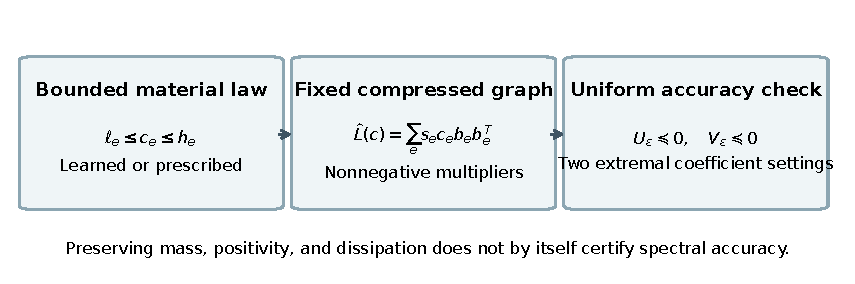
\includegraphics[width=\linewidth]{../figures/contract.pdf}
\caption{A coefficient-envelope contract. The same conductance vector enters both operators. The two extremal settings depend on the multipliers and requested tolerance. A separate bounded constitutive architecture can ensure that its predictions lie inside the envelope. The schematic was implemented in Matplotlib using plotting code developed with OpenAI Codex (GPT-6-based assistant, accessed 17 October 2026).}\label{fig:contract}
\end{figure}

\section{Related work and contribution boundary}
\paragraph{Spectral sparsification.}
Spielman and Srivastava construct sparsifiers using effective-resistance sampling \cite{ss}; Batson, Spielman, and Srivastava establish linear-sized sparsifiers \cite{bss}. These results preserve all quadratic forms of a supplied weighted graph. Recent work develops instance-dependent sparsification for sums of general positive-semidefinite matrices \cite{basu}. Our formulation uses the same spectral order, but requires one multiplier vector to work throughout a coefficient box. We do not improve classical sparsity or construction-time guarantees. Our experimental support generator is a spanning-tree-plus-leverage heuristic; it is not an implementation of the Spielman--Srivastava sampling theorem.

\paragraph{Robust matrix inequalities.}
Interval-uncertain LMIs and their tractable approximations have a substantial literature \cite{bental}. Here every uncertain direction is a signed multiple of a fixed positive-semidefinite matrix. Selecting its maximizing endpoint gives an attained Loewner upper bound. The two-envelope test is an elementary specialization of this order structure. The contribution is its explicit use for shared-coefficient compression, together with refitting, support obstructions, constructive diagnostics, and a finite empirical study. We do not claim that monotonicity or semidefinite epigraphs are new mathematics.

\paragraph{Compatible learned operators and hyper-reduction.}
Data-driven exterior calculus learns metric information while retaining conservation and exact-sequence structure \cite{trask}. Energy-based sampling and weighting \cite{farhat}, gradient-preserving DEIM \cite{pagliantini}, and entropy-stable reduced models \cite{chan} show why operator structure should survive reduction. Liljegren-Sailer studies compression of empirical-quadrature training data \cite{liljegren}. Those contributions concern compatible models and efficient approximation, with their own error analyses. We isolate a different guarantee: uniform relative energy accuracy of fixed edge multipliers under independent scalar coefficient variation. We keep all vertices and therefore perform operator compression, not state-space dimension reduction. General finite-element stiffness matrices with signed local contributions or non-diagonal learned Hodge stars are outside the graph setting unless a suitable positive-semidefinite scalar decomposition is supplied.

\paragraph{Applications and adjacent graph learning.}
Circuit-oriented support-graph preconditioning already demonstrates an industrial role for graph sparsification \cite{zhao}. Spectrum-preserving rewiring has also been studied for graph-neural-network prediction \cite{liang}. We do not compare against their application-specific systems or transfer their performance claims. The present evidence concerns a coefficient-envelope audit for scalar diffusion. Table~\ref{tab:position} separates the relevant objects.

\begin{table}[t]\centering\small
\caption{Positioning by guarantee, rather than by asserted superiority.}\label{tab:position}
\begin{tabular}{p{.25\linewidth}p{.31\linewidth}p{.34\linewidth}}\toprule
Approach & Principal object & Relation to this work\\\midrule
Classical sparsification & All states of one weighted graph & We additionally quantify over a box of conductances\\
Compatible learned graph & Conservation and compatible operators & We audit compression accuracy separately\\
Positive hyper-reduction & Efficient, structured nonlinear evaluation & We hold support fixed and certify a specified scalar envelope\\
Robust LMI methods & Uncertain matrix constraints & We exploit sign-definite directions and shared coefficients\\\bottomrule
\end{tabular}
\end{table}

\section{Model and uniform accuracy contract}
Let $G=(V,E)$ be a connected undirected graph with $n$ vertices and $m$ edges. Choose an orientation and let $b_e\in\R^n$ be the signed incidence vector of edge $e$. Write $A_e=b_eb_e^T\succeq0$. Conductances belong to the box
\begin{equation}
\mathcal C=[\ell,h]=\{c\in\R^m:0<\ell_e\le c_e\le h_e\}.
\end{equation}
Given fixed multipliers $s_e\ge0$, define
\begin{equation}\label{eq:operators}
L(c)=\sum_{e=1}^m c_eA_e,
\qquad \Lo(c)=\sum_{e=1}^m s_ec_eA_e.
\end{equation}
The support $S$ requires $s_e=0$ for $e\notin S$. The multipliers cannot adapt to $c$ in this contract. A fixed multiplier on a retained edge scales that edge's current conductance, not its conductance at a training setting.

The uniform relative energy error is
\begin{equation}\label{eq:error}
\mathcal E(s;\mathcal C)=\sup_{c\in\mathcal C}\sup_{x\notin\operatorname{span}\{\one\}}
\frac{|x^T(\Lo(c)-L(c))x|}{x^TL(c)x}.
\end{equation}
Connectivity and $\ell>0$ make the denominator positive on the quotient by constants. An equivalent contract at tolerance $\eps\ge0$ is
\begin{equation}\label{eq:contract}
(1-\eps)L(c)\preceq\Lo(c)\preceq(1+\eps)L(c)
\quad\text{for every }c\in\mathcal C.
\end{equation}
Errors above one are meaningful measures of distortion, but no longer supply a positive lower spectral bound. They do not imply that the compressed diffusion is physically unstable.

A bounded learned edge law can take the form
\begin{equation}\label{eq:learned}
c_{\theta,e}(z)=\ell_e+(h_e-\ell_e)\sigma(f_\theta(\xi_e,z)),
\end{equation}
where $\sigma$ is logistic, $z$ is an external parameter, and $\xi_e$ contains local geometry. Any parameter update leaves the output in the box. Equation~\eqref{eq:contract} therefore survives such an update without retraining $s$. This certifies compression relative to $L(c_\theta)$; it does not certify that the learned law matches the physical system. When the learned field occupies a correlated low-dimensional subset of the box, box uniformity can be conservative.

\section{Two extremal settings and exact convex refitting}
For a scalar $d$, define
\begin{equation}\label{eq:phi}
\phi_e(d)=\ell_ed+(h_e-\ell_e)\max\{d,0\}.
\end{equation}
This is the maximum of $d c_e$ over the edge interval. Define the two violation envelopes
\begin{equation}\label{eq:envelopes}
U_\eps(s)=\sum_e\phi_e(s_e-1-\eps)A_e,
\quad
V_\eps(s)=\sum_e\phi_e(1-\eps-s_e)A_e.
\end{equation}

\begin{theorem}[Two-envelope characterization]\label{thm:two}
The uniform contract \eqref{eq:contract} holds if and only if
\begin{equation}\label{eq:test}
U_\eps(s)\preceq0,\qquad V_\eps(s)\preceq0.
\end{equation}
An upper extremal setting is
\begin{equation}\label{eq:corners}
c_e^+=\begin{cases}h_e&s_e>1+\eps,\\\ell_e&s_e\le1+\eps,\end{cases}
\quad
c_e^-=\begin{cases}h_e&s_e<1-\eps,\\\ell_e&s_e\ge1-\eps.\end{cases}
\end{equation}
These settings attain $U_\eps=\Lo(c^+)-(1+\eps)L(c^+)$ and $V_\eps=(1-\eps)L(c^-)-\Lo(c^-)$.
\end{theorem}
\begin{proof}
For every admissible $c$, $(s_e-1-\eps)c_e\le\phi_e(s_e-1-\eps)$. Multiplying this scalar inequality by $A_e\succeq0$ and summing proves
$\Lo(c)-(1+\eps)L(c)\preceq U_\eps(s)$. Every coefficient is simultaneously maximized by $c^+$, so the bound is attained as a matrix, not only for a selected vector. Thus the upper contract is equivalent to $U_\eps\preceq0$. Apply the identical argument to $(1-\eps-s_e)c_e$ for the lower contract. At zero signed coefficient either endpoint is valid.
\end{proof}

The extremal settings depend on both $s$ and $\eps$. Checking the all-low and all-high settings does not replace this test: those two uniform scalings have exactly the same relative error when $h=\kappa\ell$, and can miss mixed material changes. No simultaneous diagonalization or commuting-edge assumption is used. The same proof applies to any fixed collection $A_e\succeq0$ with independent scalar intervals.

\paragraph{Constructive failure and numerical evaluation.}
Let $Q\in\R^{n\times(n-1)}$ have orthonormal columns spanning $\one^\perp$. We test $Q^TU_\eps Q$ and $Q^TV_\eps Q$. A positive eigenpair $(\lambda,y)$ gives a witness $x=Qy$ and one explicit corner from \eqref{eq:corners} where the requested contract fails. For fixed $s$, feasibility is monotone in $\eps$. Bisection brackets $\mathcal E$; $\max\{1,\max_es_e-1\}$ is a valid upper endpoint because $0\preceq\Lo(c)\preceq(\max_es_e)L(c)$. The artifact uses 48 iterations and additionally computes generalized eigenvalues at the final extremal settings to report an attained distortion.

\begin{proposition}[Exact fixed-support refit]\label{prop:sdp}
Minimizing \eqref{eq:error} over nonnegative multipliers supported on $S$ has the following convex semidefinite formulation:
\begin{align}\label{eq:sdp}
\min_{s,p,q,\eps}\quad &\eps\\
\text{subject to}\quad &s,p,q,\eps\ge0,\quad s_e=0\ (e\notin S),\nonumber\\
&p_e\ge s_e-1-\eps,\quad q_e\ge1-\eps-s_e,\nonumber\\
&\sum_e[\ell_e(s_e-1-\eps)+(h_e-\ell_e)p_e]Q^TA_eQ\preceq0,\nonumber\\
&\sum_e[\ell_e(1-\eps-s_e)+(h_e-\ell_e)q_e]Q^TA_eQ\preceq0.\nonumber
\end{align}
\end{proposition}
\begin{proof}
For any feasible epigraph variables, $p_e\ge\max(s_e-1-\eps,0)$ and the analogous bound holds for $q_e$. Since $(h_e-\ell_e)A_e\succeq0$, the matrix expressions in \eqref{eq:sdp} dominate the corresponding violation envelopes. Their nonpositivity implies \eqref{eq:test}. Conversely, whenever \eqref{eq:test} holds, choosing the positive parts exactly makes \eqref{eq:sdp} feasible. All constraints in this lifted formulation are affine or conic, including their dependence on $\eps$.
\end{proof}

There are two semidefinite blocks of order $n-1$ and $O(m)$ scalar variables, independent of the number of box corners. Support selection remains combinatorial and is not solved by this proposition. The dense reference implementation materializes edge outer products for the SDP, requiring $O(mn^2)$ storage. Certification need only assemble two Laplacian sums and solve two symmetric eigenproblems per tolerance. Neither observation provides a nearly linear-time construction claim.

\section{Limits imposed by omitted interactions}
\begin{theorem}[Support obstruction]\label{thm:omit}
Let $D=\sum_{e\notin S}(h_e-\ell_e)A_e$ and $L_0=L(\ell)$. Let
\begin{equation}
\delta_S=\lambda_{\max}(Q^TDQ,Q^TL_0Q).
\end{equation}
Every multiplier vector supported on $S$ obeys
\begin{equation}\label{eq:lower}
\mathcal E(s;\mathcal C)\ge\frac{\delta_S}{2+\delta_S}.
\end{equation}
\end{theorem}
\begin{proof}
At $c=\ell$ and at the corner obtained by raising only omitted conductances to $h$, the compressed operator is identical. The full operators are $L_0$ and $L_0+D$. If both satisfy tolerance $\eps$, then
$(1-\eps)(L_0+D)\preceq\Lo(\ell)\preceq(1+\eps)L_0$.
Hence $(1-\eps)D\preceq2\eps L_0$. For $\eps<1$, evaluation on a maximizing generalized eigenvector gives $(1-\eps)\delta_S\le2\eps$ and \eqref{eq:lower}. For $\eps\ge1$, the bound follows directly because its right-hand side is less than one.
\end{proof}

This obstruction holds regardless of how retained weights are fitted. For $h=\kappa\ell$, one omitted edge gives the weaker but inexpensive necessary bound with $\delta=(\kappa-1)\ell_e b_e^TL_0^\dagger b_e$. The collective omitted-set bound can be stronger. If at least one edge is omitted and its allowed range grows without bound while retained lower bounds remain fixed, the lower bound tends to one. A fixed sparse support cannot promise uniformly small distortion over arbitrarily strong independent coefficient changes. The bound is necessary, not generally sufficient or tight.

\begin{corollary}[Closed-form scalar minimax refit]\label{cor:scalar}
Assume $h=\kappa\ell$, $\kappa\ge1$, and let $s=\alpha\one_S$ with $\alpha\ge0$. Set $T=\sum_{e\in S}\ell_eA_e$. Let $t_{\min},t_{\max}$ be the smallest and largest generalized eigenvalues of $(Q^TTQ,Q^TL_0Q)$, and define
\begin{equation}
a=\frac{t_{\min}}{\kappa-(\kappa-1)t_{\min}},\qquad
b=\frac{\kappa t_{\max}}{1+(\kappa-1)t_{\max}}.
\end{equation}
If $a+b>0$, a minimax scalar and its exact error are
\begin{equation}\label{eq:scalar}
\alpha_*=\frac{2}{a+b},\qquad\eps_*^{\mathrm{scalar}}=\frac{b-a}{b+a}.
\end{equation}
If $T=0$, the minimum error is one.
\end{corollary}
\begin{proof}
For fixed $x$, the ratio $\alpha x^TT(c)x/[x^TT(c)x+x^TD(c)x]$ increases with every retained conductance and decreases with every omitted conductance. Its global minimum is the smallest generalized eigenvalue of $(\alpha T,T+\kappa(L_0-T))$; its maximum is the largest generalized eigenvalue of $(\alpha\kappa T,\kappa T+L_0-T)$. Congruence by the inverse square root of $L_0$ turns these into the increasing scalar functions of $t$ displayed above. The entire ratio range is bounded by $\alpha a$ and $\alpha b$, and both endpoints are attained. Thus the error is $\max\{1-\alpha a,\alpha b-1\}$. Balancing the two terms gives \eqref{eq:scalar}. If $a=0<b$, this choice is one of possibly many minimizers with error one.
\end{proof}

\paragraph{An exact triangle example.}
Take the unit-weight triangle and retain a two-edge path. The nominal generalized eigenvalues are $1/3$ and $1$. Therefore $\alpha_*=(1+2\kappa)/(1+\kappa)$ and $\eps_*=\kappa/(1+\kappa)$. These values are also optimal among separate nonnegative weights on the two retained edges: swapping the path endpoints preserves the full problem, and averaging a feasible solution with its swapped copy preserves feasibility of the convex refit. Nominal fitting instead selects $\alpha=3/2$ and has box error $\max\{1/2,1-3/[2(1+2\kappa)]\}$. At contrast four, box fitting improves $5/6$ to $4/5$; the remaining error is still large. This small example makes the limitation of reweighting concrete.

\section{Physical structure and switched diffusion error}
Let $M$ be a fixed positive diagonal capacity matrix. At time step $k$ let $L_k=L(c^k)$ and $H_k=\Lo(c^k)$, with the \emph{same externally prescribed} coefficient vector used in the two systems. For step size $\tau>0$, define
\begin{equation}\label{eq:be}
(M+\tau L_k)u^{k+1}=Mu^k,\qquad
(M+\tau H_k)v^{k+1}=Mv^k.
\end{equation}
There are no source terms or boundary fluxes. Nonnegative multipliers ensure that the second system preserves weighted mass, maps nonnegative data to nonnegative data, and dissipates $E(v)=\tfrac12v^TMv$. Indeed, $H_k\one=0$, and $M+\tau H_k$ is a strictly diagonally dominant symmetric M-matrix. Its inverse is nonnegative. Multiplying the discrete equation by $v^{k+1}$ gives
\begin{equation}\label{eq:energy}
E(v^{k+1})-E(v^k)+\tfrac12\norm{v^{k+1}-v^k}_M^2
+\tau(v^{k+1})^TH_kv^{k+1}=0.
\end{equation}
These standard structural facts hold even when the spectral approximation is poor.

\begin{theorem}[Uniform switched backward-Euler error]\label{thm:dyn}
Suppose $u^0=v^0$, and $(1-\eps)L_k\preceq H_k\preceq(1+\eps)L_k$ for every $k$, with $0\le\eps<1$. Then for every number of steps $N$,
\begin{equation}\label{eq:dynbound}
\norm{v^N-u^N}_M^2\le \frac{\eps^2}{1-\eps}E(u^0).
\end{equation}
The same inequality holds with $E(u^0)$ replaced by $E(u^0-\bar u\one)$, where $\bar u=(\one^TMu^0)/(\one^TM\one)$.
\end{theorem}
\begin{proof}
Let $e^k=v^k-u^k$ and $\Delta_k=H_k-L_k$. Subtraction in \eqref{eq:be} gives
$M(e^{k+1}-e^k)/\tau+H_ke^{k+1}=-\Delta_ku^{k+1}$.
The spectral contract implies the bilinear estimate
$|x^T\Delta_ky|\le\eps\sqrt{x^TL_kx}\sqrt{y^TL_ky}$ on the quotient by constants, by applying the operator norm bound to $L_k^{-1/2}\Delta_kL_k^{-1/2}$. Testing by $e^{k+1}$ and applying Young's inequality yields
\[
\frac{\norm{e^{k+1}}_M^2-\norm{e^k}_M^2}{2\tau}
+\frac{1-\eps}{2}(e^{k+1})^TL_ke^{k+1}
\le\frac{\eps^2}{2(1-\eps)}(u^{k+1})^TL_ku^{k+1}.
\]
The discarded increment norm is nonnegative. Summing and using the full-model identity \eqref{eq:energy} gives
$\sum_k\tau(u^{k+1})^TL_ku^{k+1}\le E(u^0)$ and proves \eqref{eq:dynbound}. Subtracting the conserved common mean leaves every Laplacian term and the error unchanged, proving the final assertion.
\end{proof}

No temporal smoothness of $c^k$ is required. Common positive scalar rescaling $c^k=\gamma_k\widetilde c^k$, $\gamma_k>0$, $\widetilde c^k\in\mathcal C$, also retains the contract by homogeneity. The estimate is deliberately coarse and can be much larger than the observed error. It does not cover a nonlinear rollout that evaluates $c(u^k)$ in one system and $c(v^k)$ in the other; that comparison requires additional constitutive regularity and stability analysis. Positivity of a general reduced-coordinate Galerkin model is also not implied.

\section{Reproducible experimental design}
The study asks three separate questions: whether the characterization is implemented correctly; whether robust refitting improves the specified worst-case objective; and what this costs on typical learned coefficient settings. All graphs and observations are synthetic. The protocol, graph definitions, parameters, multipliers, per-fit results, and plotting code are included in the artifact.

\paragraph{Graph families and supports.}
We use 16 vertices in four families: a $4\times4$ grid including diagonal neighbors (42 edges); a five-nearest-neighbor geometric graph augmented by a vertex chain (57 edges); two eight-vertex cliques connected by two edges (58 edges); and the complete graph (120 edges). Vertex coordinates and exact edge lists are saved. Lower conductances are $\ell_e=0.6+\exp(-2d_e)$, with $d_e$ the Euclidean edge length. For each seed in $\{101,202,303,404\}$, a maximum-$\ell$ spanning tree is retained first. Remaining edges are ordered by independent exponential keys with rates equal to nominal effective-resistance leverage scores. A prefix supplies each requested retained fraction $\rho\in\{0.5,0.75,0.9\}$, rounded up and never below $n-1$. All fitting methods share the same support in each comparison. We test $\kappa\in\{1,2,4,8\}$ and $h=\kappa\ell$, giving 192 graph--seed--budget--contrast cells.

\paragraph{An actually trained bounded constitutive field.}
For each graph, a six-input, 16-hidden-unit tanh network with logistic output is trained to regress a manufactured material law. Inputs are twice the centered edge midpoint coordinates, squared coordinate differences of the endpoints, and two external parameters $z\in[-1,1]^2$. More precisely the midpoint inputs are $a=2\xi_x-1$, $b=2\xi_y-1$; the other geometric inputs are $d_x^2,d_y^2$. The normalized teacher conductance is
\begin{equation}
y(\xi,z)=\sigma\!\left(1.1\sin(2a+z_1)+0.8\cos(2b-z_2)+0.6z_1z_2+d_x^2-d_y^2-0.4\right).
\end{equation}
We draw 128 training parameter vectors and 128 independent test parameter vectors using seed 411, and train all network parameters with L-BFGS-B for at most 400 iterations. The objective is mean squared normalized-conductance error plus $10^{-7}\norm{\theta}_2^2$. All four runs reach the iteration limit; they are not reported as converged optimizers. Their held-out normalized RMSE ranges from 0.00265 to 0.00339. The field supplies realistic correlation for the mechanism study, not an industrial dataset or an architectural contribution. Its output enters \eqref{eq:learned}.

\paragraph{Three fitting objectives.}
The nominal baseline minimizes relative spectral distortion at the interval midpoint. The scenario baseline minimizes the maximum distortion over eight parameter settings drawn from the fitted neural field. The box method solves \eqref{eq:sdp}. The first two use the same nonnegative supported multipliers and ordinary per-scenario spectral LMIs; thus no structural advantage is reserved for the box method. The eight fitting settings, 128 held-out learned settings, and 128 independent uniform box settings are generated by each support seed and shared across methods and contrasts within the cell. We record the maximum over each held-out set, the exact-box numerical certificate, and solver status. The finite-scenario objective is not a distribution-free robust guarantee.

\paragraph{Software and numerical verification.}
Experiments use Python 3.9.6, NumPy 1.26.4, SciPy 1.13.1, CVXPY 1.7.5 \cite{cvxpy}, and Clarabel 0.11.1 \cite{clarabel}, on arm64 macOS. Thread counts are fixed to one. Solver absolute feasibility and gap tolerances are $10^{-8}$. We independently re-evaluate every fitted multiplier vector using the two-envelope test, rather than interpreting a solver status as a certificate. Forty-seven of 576 solves report \texttt{optimal\_inaccurate}; all statuses are retained. Among the 192 box fits, the largest difference between the solver objective and the independent envelope recheck is $3.77\times10^{-8}$. This is numerical agreement, not an exact-arithmetic proof of each fitted instance. Theorems are stated in real arithmetic; the implementation does not use interval eigensolvers.

\paragraph{Research and visualization tooling.}
OpenAI Codex (OpenAI; GPT-6-based assistant, accessed 17 October 2026) assisted research formulation, mathematical development, implementation, execution and analysis, and plotting-code development. Numerical results were obtained by running the supplied Python scripts. Matplotlib figures reproduce the saved outputs and analytical formulas; no measurements were supplied by a language model. Code, parameters, results, and figure scripts are publicly available for inspection.

\section{Results}
\subsection{Finite validation of the certificate}
For 120 random multiplier/interval instances on $K_4$, we enumerate all $2^6=64$ coefficient corners: 7,680 corner evaluations. The largest difference between enumeration and the two-envelope certificate is $8.0\times10^{-15}$. A separate verifier constructs full Laplacians by direct entry updates, grounds one vertex, and uses a Cholesky congruence to compute quotient eigenvalues. It imports neither the core incidence assembly nor the core relative-error function. Its additional 60 instances cover 3,840 corner evaluations and agree to nine decimal places. These are finite implementation checks; the characterization for all graphs follows from Theorem~\ref{thm:two}.

The test suite also covers zero compression, the identity multipliers, disconnected supports, invalid intervals, negative multipliers, the support lower bound, convex refitting, and 12 scalar-formula settings. Six test methods pass. Counts distinguish design instances from individual corner evaluations; they are not independent draws from a real deployment population.

\subsection{Worst-case accuracy and its empirical cost}
Table~\ref{tab:aggregate} averages over the 48 graph--seed--budget cells at each contrast. At $\kappa=1$, all three objectives coincide up to solver precision. At larger contrast, the box objective improves on nominal fitting in all 144 paired cells by more than $10^{-6}$. That direction is expected because nominally fitted weights are feasible candidates for the robust minimization; the experiment quantifies the size of the tradeoff, rather than establishing the existence of that ordering. At contrast eight the ratio of aggregate means decreases by 32.8\%, from 1.260 to 0.847.

\begin{table}[t]\centering\small
\caption{Mean errors over 48 cells per contrast. ``Learned test maximum'' is the maximum over 128 held-out learned parameter settings within each cell, then averaged over cells. All entries are relative quadratic-form errors, not prediction RMSE.}\label{tab:aggregate}
\begin{tabular}{lrrrrrr}\toprule
&\multicolumn{3}{c}{Box worst case}&\multicolumn{3}{c}{Learned test maximum}\\
$\kappa$ & Nominal & Scenario & Box & Nominal & Scenario & Box\\\midrule
1 & 0.404 & 0.404 & 0.404 & 0.404 & 0.404 & 0.404\\
2 & 0.701 & 0.714 & 0.593 & 0.435 & 0.425 & 0.541\\
4 & 0.991 & 1.019 & 0.741 & 0.463 & 0.446 & 0.674\\
8 & 1.260 & 1.317 & 0.847 & 0.484 & 0.463 & 0.776\\
\bottomrule\end{tabular}

\end{table}

\begin{figure}[t]\centering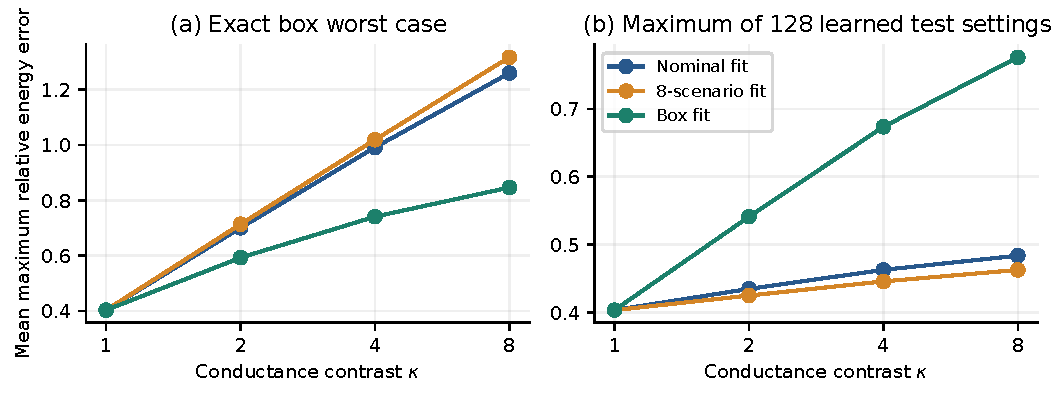
\includegraphics[width=\linewidth]{../figures/contrast.pdf}
\caption{The observed tradeoff. Curves average over all four graph families, four support seeds, and three budgets. Box fitting improves its uniform objective while worsening the maximum on ordinary learned test settings. No confidence intervals over a deployment population are implied.}\label{fig:contrast}
\end{figure}

The improved worst-case bound is not a general empirical advantage. At $\kappa=8$, the mean learned-test maximum rises from 0.484 for nominal fitting to 0.776 for box fitting. Scenario fitting attains 0.463 on that same test criterion but has mean box worst case 1.317. The box includes independently varying edge coefficients that the two-parameter learner does not generate. Paying for those settings can shift weights away from the learned manifold. This is evidence for explicitly choosing the deployment envelope, not for treating a larger envelope as cost-free robustness.

Figure~\ref{fig:sampling} compares sampled maxima with exact-box values. Sampling 128 independent box settings still misses important extremal combinations for many nominal fits. The learned test sample is even more restricted. These observations motivate the exact check but do not establish a universal sample-complexity lower bound.

\begin{figure}[t]\centering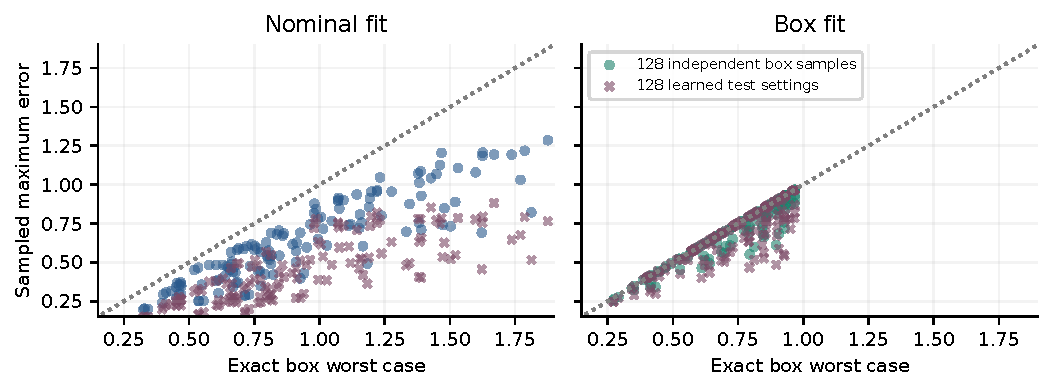
\includegraphics[width=\linewidth]{../figures/sampling.pdf}
\caption{Sampling can underestimate the declared box worst case. Each panel has 144 cells with $\kappa>1$. The dotted line denotes equality. Independent box samples and correlated learned settings answer different questions.}\label{fig:sampling}
\end{figure}

\subsection{Graph dependence and edge budgets}
Table~\ref{tab:families} holds the requested retained fraction at 0.75 and contrast at four. The complete graph tolerates compression better than the local grid in this finite study. However, substantial distortion remains even after robust refitting. Figure~\ref{fig:budget} shows that more retained edges usually improve the attainable uniform approximation, with topology and support selection affecting the result. The plots report means and seed ranges, not inferential uncertainty. We neither optimize the support globally nor claim a minimum edge count from these curves.

\begin{table}[t]\centering\small
\caption{Numerically certified box error at requested fraction 0.75 and $\kappa=4$. Values are mean $\pm$ sample standard deviation over four support seeds. Retained counts are rounded up.}\label{tab:families}
\begin{tabular}{lrrlll}\toprule
Graph & Edges & Retained & Nominal & Scenario & Box\\\midrule
Grid & 42 & 32 & $0.956 \pm 0.091$ & $0.902 \pm 0.093$ & $0.805 \pm 0.014$\\
Geometric & 57 & 43 & $0.936 \pm 0.127$ & $0.925 \pm 0.100$ & $0.769 \pm 0.033$\\
Clustered & 58 & 44 & $1.071 \pm 0.079$ & $1.114 \pm 0.310$ & $0.815 \pm 0.050$\\
Complete & 120 & 90 & $0.707 \pm 0.057$ & $0.834 \pm 0.255$ & $0.650 \pm 0.048$\\
\bottomrule\end{tabular}

\end{table}

\begin{figure}[t]\centering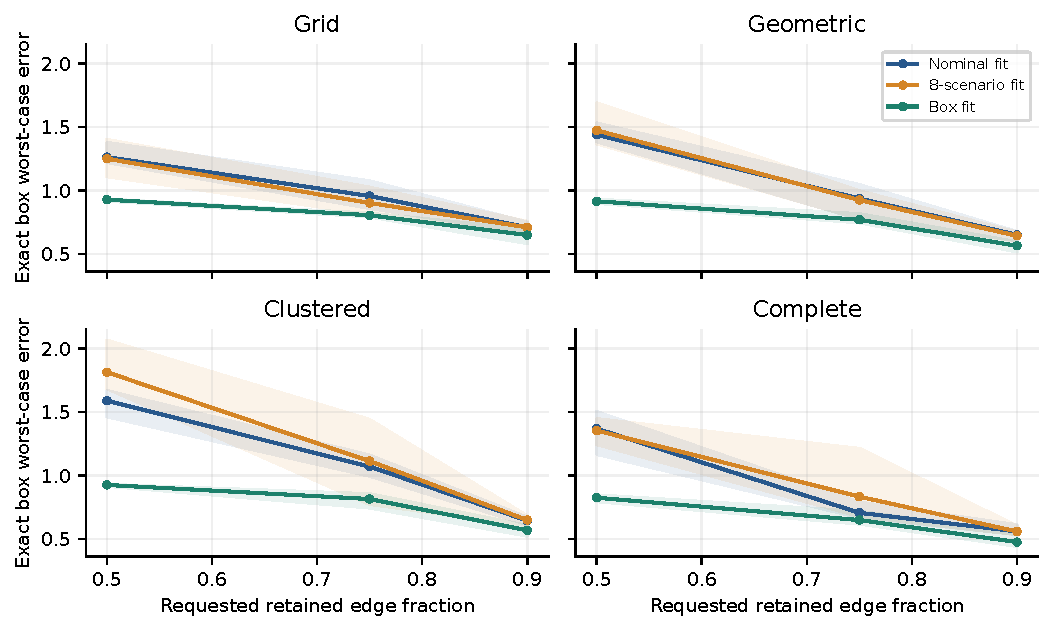
\includegraphics[width=.9\linewidth]{../figures/budget.pdf}
\caption{Uniform distortion versus retained fraction at contrast four. Lines show four-seed means and bands show the full seed range. A connected, physically dissipative compressed graph can still have substantial approximation error.}\label{fig:budget}
\end{figure}

\subsection{Switched diffusion checks and larger scalar refits}
For each graph, seed 101, fraction 0.75, and contrast four, we simulate all three fitted models at their own attained worst spectral setting. The common time-dependent coefficient factor is $1+0.25\sin(0.31k)$; homogeneity preserves the spectral ratio under this global rescaling. Each run uses 100 backward-Euler steps of size 0.04, seeded nonnegative initial states, and capacities sampled uniformly in $[0.7,1.3]$. Across the 12 compressed runs, the maximum weighted-mass drift is $1.45\times10^{-14}$; the largest upward energy increment is $1.34\times10^{-15}$; all state values remain positive. Every run with a spectral error below one satisfies Theorem~\ref{thm:dyn}. The bounds are loose: for the four box fits, observed maximum state errors lie between 0.159 and 0.196, whereas the uncentered energy bounds lie between 2.46 and 3.14. These checks verify a numerical consequence of the contract, not superior trajectory accuracy. Each method's different worst-case coefficient setting also prevents interpreting the runs as a common-input performance ranking.

We additionally execute 216 closed-form scalar refits on complete and eight-nearest-neighbor-plus-chain geometric graphs with 32, 64, and 128 vertices, three seeds, three budgets, and four contrasts. The largest complete graph has 8,128 edges. Figure~\ref{fig:limits} combines this study with the exact triangle example. These larger experiments use Corollary~\ref{cor:scalar}; they are not evidence that the dense per-edge SDP scales to 128 vertices with a large edge count.

\begin{figure}[t]\centering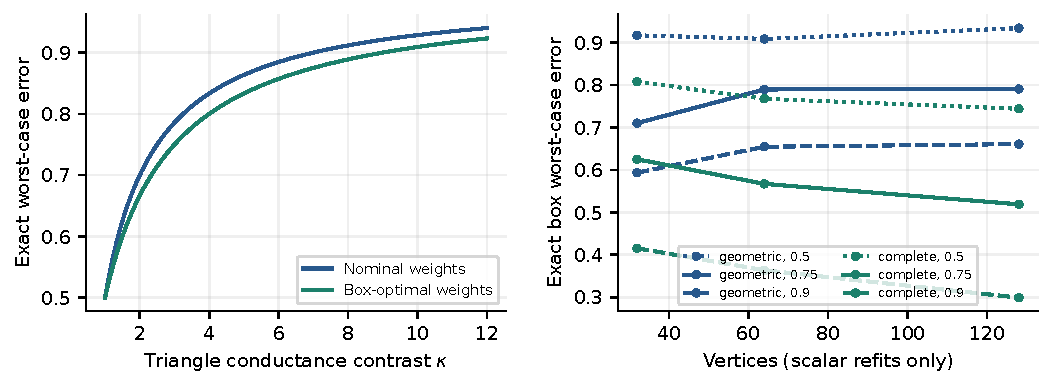
\includegraphics[width=\linewidth]{../figures/limits.pdf}
\caption{Compression limits at two scales. Left: exact analytical triangle curves; right: executed scalar refits at contrast four, averaged over three support seeds. Scalar refitting restricts all retained edges to one multiplier and need not match the per-edge SDP optimum.}\label{fig:limits}
\end{figure}

The primary 576-fit study takes approximately 102 seconds in the recorded run. Median solver-reported times are 0.014 seconds for nominal fitting, 0.326 seconds for eight-scenario fitting, and 0.041 seconds for box fitting. These times exclude model construction, coefficient learning, and certificate rechecks. The smaller number of semidefinite blocks helps in this small dense implementation, but the numbers are not portable speedup guarantees. Removing edges reduces the count of local constitutive evaluations to $|S|$ when the law can be evaluated edgewise. We do not equate that count reduction with a measured end-to-end runtime or energy saving.

\section{Practical use and limitations}
\paragraph{A deployment decision rather than an accuracy slogan.}
An engineering workflow can first specify the tolerated relative energy distortion and admissible coefficient envelope. It then selects a support, checks the inexpensive omission bound, fits nonnegative weights, and exports the certificate together with explicit assumptions. If the certificate fails, it returns a material setting and a state direction that expose the failure. The modeler can retain more edges, revise the envelope with physical justification, or allow coefficient-adaptive recompression. The workflow should not silently shrink the envelope to obtain a favorable number.

\paragraph{Commercial relevance.}
Thermal-network surrogates, learned resistor networks, and repeated material-parameter sweeps are plausible integration settings: they already have a graph, positive local constitutive evaluations, and a reason to reuse a sparse operator. Published circuit-preconditioning work establishes an adjacent industrial use of sparsification \cite{zhao}, while compatible learned graph models establish the scientific modeling connection \cite{trask}. A concrete product capability would be an offline audit/refit component that exports supported weights and a declared coefficient range. The present study does not establish customer demand, market size, patentability, or production acceleration. A meaningful next benchmark would measure repeated calibrated-model updates on an engineering network with independently verified coefficient bounds and full deployment cost accounting.

\paragraph{Scope of the guarantee.}
The coefficient box is not learned or statistically calibrated here. Independent intervals can greatly overapproximate correlated material physics, as the observed test tradeoff demonstrates. The theorem requires fixed positive-semidefinite edge directions and shared uncertain coefficients; independently uncertain full and compressed coefficients, changing graph incidence, signed transport, non-diagonal capacities, and general advection do not satisfy these assumptions automatically. The dynamical comparison assumes a common exogenous coefficient sequence. General nonlinear state-dependent constitutive laws need additional analysis.

\paragraph{Evidence and novelty.}
The principal empirical study is deliberately small and synthetic. It establishes implementation correctness on declared finite tests, quantifies a robust-versus-typical tradeoff, and exposes limitations of fixed support. It does not establish continuum PDE convergence, a state-of-the-art neural operator, or large-scale solver superiority. The numerical verifier uses ordinary floating-point arithmetic, and some optimization statuses are inaccurate. The core two-envelope argument is elementary order reasoning related to established robust optimization; the proposed contribution is the combined compression contract, constructive audit, exact refit, support obstruction, scalar formula, and reproducible investigation. Literature searches cannot establish that no equivalent formulation exists anywhere. Publication and presentation suitability depend on independent assessment of this contribution and its scope.

\section{Conclusion}
A compressed learned diffusion network should carry two distinct statements: which physical properties it preserves, and over which constitutive coefficients it remains an accurate approximation. For fixed nonnegative edge multipliers, a box-uniform spectral contract has a simple exact characterization through two tolerance-dependent extremal settings. This makes it possible to refit weights convexly, return explicit failures, and identify support-level limitations before deployment. The experiments show both the benefit and the price of this guarantee: lower worst-case distortion and potentially higher error on ordinary learned settings. Declaring that tradeoff is essential to using structure-preserving compression responsibly.

\paragraph{Code and data availability.}
Source code, manufactured-data generators, trained parameters, raw results, tests, figures, and manuscript sources are available at \url{https://github.com/shi1720/constitutive-box}. All observations reported here are generated by the supplied scripts. The local protocol records the executed design and is not a public preregistration.

\paragraph{Author contribution.}
Shivam Gupta directed the project, reviewed and approved the final manuscript, and is the sole author and corresponding author.

\paragraph{Funding.}
This research did not receive a specific grant from funding agencies in the public, commercial, or not-for-profit sectors.

\section*{Declaration of generative AI and AI-assisted technologies in the manuscript preparation process}
During preparation, OpenAI Codex assisted with literature review, mathematical development, code, analysis, plotting, and writing. Shivam Gupta reviewed and edited the content as needed and takes full responsibility for the manuscript.

\begin{thebibliography}{99}\small
\bibitem{ss} D. A. Spielman and N. Srivastava. Graph sparsification by effective resistances. \emph{SIAM Journal on Computing}, 40(6):1913--1926, 2011. \href{https://doi.org/10.1137/080734029}{doi:10.1137/080734029}.
\bibitem{bss} J. Batson, D. A. Spielman, and N. Srivastava. Twice-Ramanujan sparsifiers. \emph{SIAM Journal on Computing}, 41(6):1704--1721, 2012. \href{https://doi.org/10.1137/090772873}{doi:10.1137/090772873}.
\bibitem{trask} N. Trask, A. Huang, and X. Hu. Enforcing exact physics in scientific machine learning: A data-driven exterior calculus on graphs. \emph{Journal of Computational Physics}, 456:110969, 2022. \href{https://doi.org/10.1016/j.jcp.2022.110969}{doi:10.1016/j.jcp.2022.110969}.
\bibitem{farhat} C. Farhat, P. Avery, T. Chapman, and J. Cortial. Dimensional reduction of nonlinear finite element dynamic models with finite rotations and energy-based mesh sampling and weighting for computational efficiency. \emph{International Journal for Numerical Methods in Engineering}, 98(9):625--662, 2014. \href{https://doi.org/10.1002/nme.4668}{doi:10.1002/nme.4668}.
\bibitem{pagliantini} C. Pagliantini and F. Vismara. Gradient-preserving hyper-reduction of nonlinear dynamical systems via discrete empirical interpolation. arXiv:2206.01792, version 2, 2023. \url{https://arxiv.org/abs/2206.01792}.
\bibitem{liljegren} B. Liljegren-Sailer. Reducing training complexity in empirical quadrature-based model reduction via structured compression. arXiv:2512.14416, 2025. \url{https://arxiv.org/abs/2512.14416}.
\bibitem{bental} A. Ben-Tal and A. Nemirovski. On tractable approximations of uncertain linear matrix inequalities affected by interval uncertainty. \emph{SIAM Journal on Optimization}, 12(3):811--833, 2002. \href{https://doi.org/10.1137/S1052623400374756}{doi:10.1137/S1052623400374756}.
\bibitem{basu} A. Basu, P. K. Kothari, Y. P. Liu, and R. Meka. Sparsifying sums of positive semidefinite matrices. In \emph{Proceedings of SODA 2026}, pp. 6042--6064, 2026. \href{https://doi.org/10.1137/1.9781611978971.216}{doi:10.1137/1.9781611978971.216}.
\bibitem{chan} J. Chan. Entropy stable reduced order modeling of nonlinear conservation laws. \emph{Journal of Computational Physics}, 423:109789, 2020. \href{https://doi.org/10.1016/j.jcp.2020.109789}{doi:10.1016/j.jcp.2020.109789}.
\bibitem{zhao} X. Zhao, L. Han, and Z. Feng. A performance-guided graph sparsification approach to scalable and robust SPICE-accurate integrated circuit simulations. \emph{IEEE Transactions on Computer-Aided Design of Integrated Circuits and Systems}, 34(10):1639--1651, 2015. \href{https://doi.org/10.1109/TCAD.2015.2424958}{doi:10.1109/TCAD.2015.2424958}.
\bibitem{liang} L. Liang, F. Bu, Z. Song, Z. Xu, S. Pan, and K. Shin. Mitigating over-squashing in graph neural networks by spectrum-preserving sparsification. In \emph{Proceedings of ICML}, PMLR 267, 2025. \url{https://arxiv.org/abs/2506.16110}.
\bibitem{cvxpy} S. Diamond and S. Boyd. CVXPY: A Python-embedded modeling language for convex optimization. \emph{Journal of Machine Learning Research}, 17(83):1--5, 2016. \url{https://www.jmlr.org/papers/v17/15-408.html}.
\bibitem{clarabel} P. J. Goulart and Y. Chen. Clarabel: An interior-point solver for conic programs with quadratic objectives. arXiv:2405.12762, 2024. \url{https://arxiv.org/abs/2405.12762}.
\end{thebibliography}

\appendix
\section{Reproduction map}
From the repository root, install \texttt{requirements.txt} in a fresh virtual environment, then run:
\begin{lstlisting}
OPENBLAS_NUM_THREADS=1 OMP_NUM_THREADS=1 VECLIB_MAXIMUM_THREADS=1 python experiments/run.py
OPENBLAS_NUM_THREADS=1 python experiments/scaling.py
python -m unittest discover -s tests -v
python experiments/figures.py
cd paper
tectonic main.tex
\end{lstlisting}
The manuscript uses vector PDF figures. Tectonic is required only for rebuilding the manuscript, not for reproducing the mathematics or experiments. Runtime and solver timings vary by environment. Saved JSON contains the original run; rerunning regenerates numerical results and timing fields.

\begin{center}\small
\begin{tabular}{p{.42\linewidth}p{.48\linewidth}}\toprule
Path & Contents\\\midrule
\texttt{src/constitutive\_box.py} & Certificate, witness, robust refit, scalar formula, omission bound\\
\texttt{experiments/protocol.json} & Main executed finite design\\
\texttt{experiments/run.py} & Learned-field training and 576-fit study\\
\texttt{results/study.json} & Every support, multiplier vector, metric, and solver status\\
\texttt{results/exhaustive.json} & All 120 corner-enumeration designs\\
\texttt{results/learned\_*.npz} & Trained network parameters and parameter splits\\
\texttt{results/dynamics.json} & Coefficient witnesses and 12 state-error/energy trajectories\\
\texttt{experiments/scaling.py} & Larger scalar-refit experiment\\
\texttt{tests/test\_certificates.py} & Independent grounded assembly and boundary checks\\
\texttt{experiments/figures.py} & Figures and manuscript tables from saved results\\\bottomrule
\end{tabular}
\end{center}

\section{Minimal certificate example}
\begin{lstlisting}
import numpy as np
from constitutive_box import Graph, certify, scalar_fit

# A triangle, retaining the first two edges (a connected path).
g = Graph(np.array([[0, 1], [1, 2], [0, 2]]), 3)
lo = np.ones(3)
keep = np.array([True, True, False])
s, exact = scalar_fit(g, lo, keep, kappa=4)
certificate = certify(g, lo, 4*lo, s)
assert abs(exact - 0.8) < 1e-10
assert abs(certificate['epsilon'] - exact) < 1e-9
print(s, certificate['witness_c'])
\end{lstlisting}
The witness conductances and state returned by \texttt{certify} attain the reported error to floating-point tolerance. A formal deployment certificate would additionally require validated bounds on numerical eigenvalues and on the supplied constitutive intervals.
\end{document}
